\chapter{Conception du Système d'Enchères}

\section{Architecture Globale}
Ce chapitre présente l'architecture et la conception détaillée du système d'enchères d'automobiles. Notre approche de conception suit les principes de l'architecture client-serveur moderne, optimisée pour les applications en temps réel avec des exigences élevées en matière de réactivité et de fiabilité.

\subsection{Vue d'ensemble}
Le système est structuré selon une architecture à plusieurs couches comprenant:
\begin{itemize}
    \item Une application mobile frontend développée avec React Native
    \item Un backend serveur RESTful basé sur Node.js et Express
    \item Une couche de communication en temps réel utilisant Socket.io
    \item Une base de données MongoDB pour le stockage persistant
\end{itemize}

\section{Diagramme de Cas d'Utilisation}
Le diagramme de cas d'utilisation ci-dessous illustre les principales fonctionnalités du système du point de vue des acteurs principaux: l'utilisateur standard et l'administrateur.

\begin{figure}[h]
    \centering
    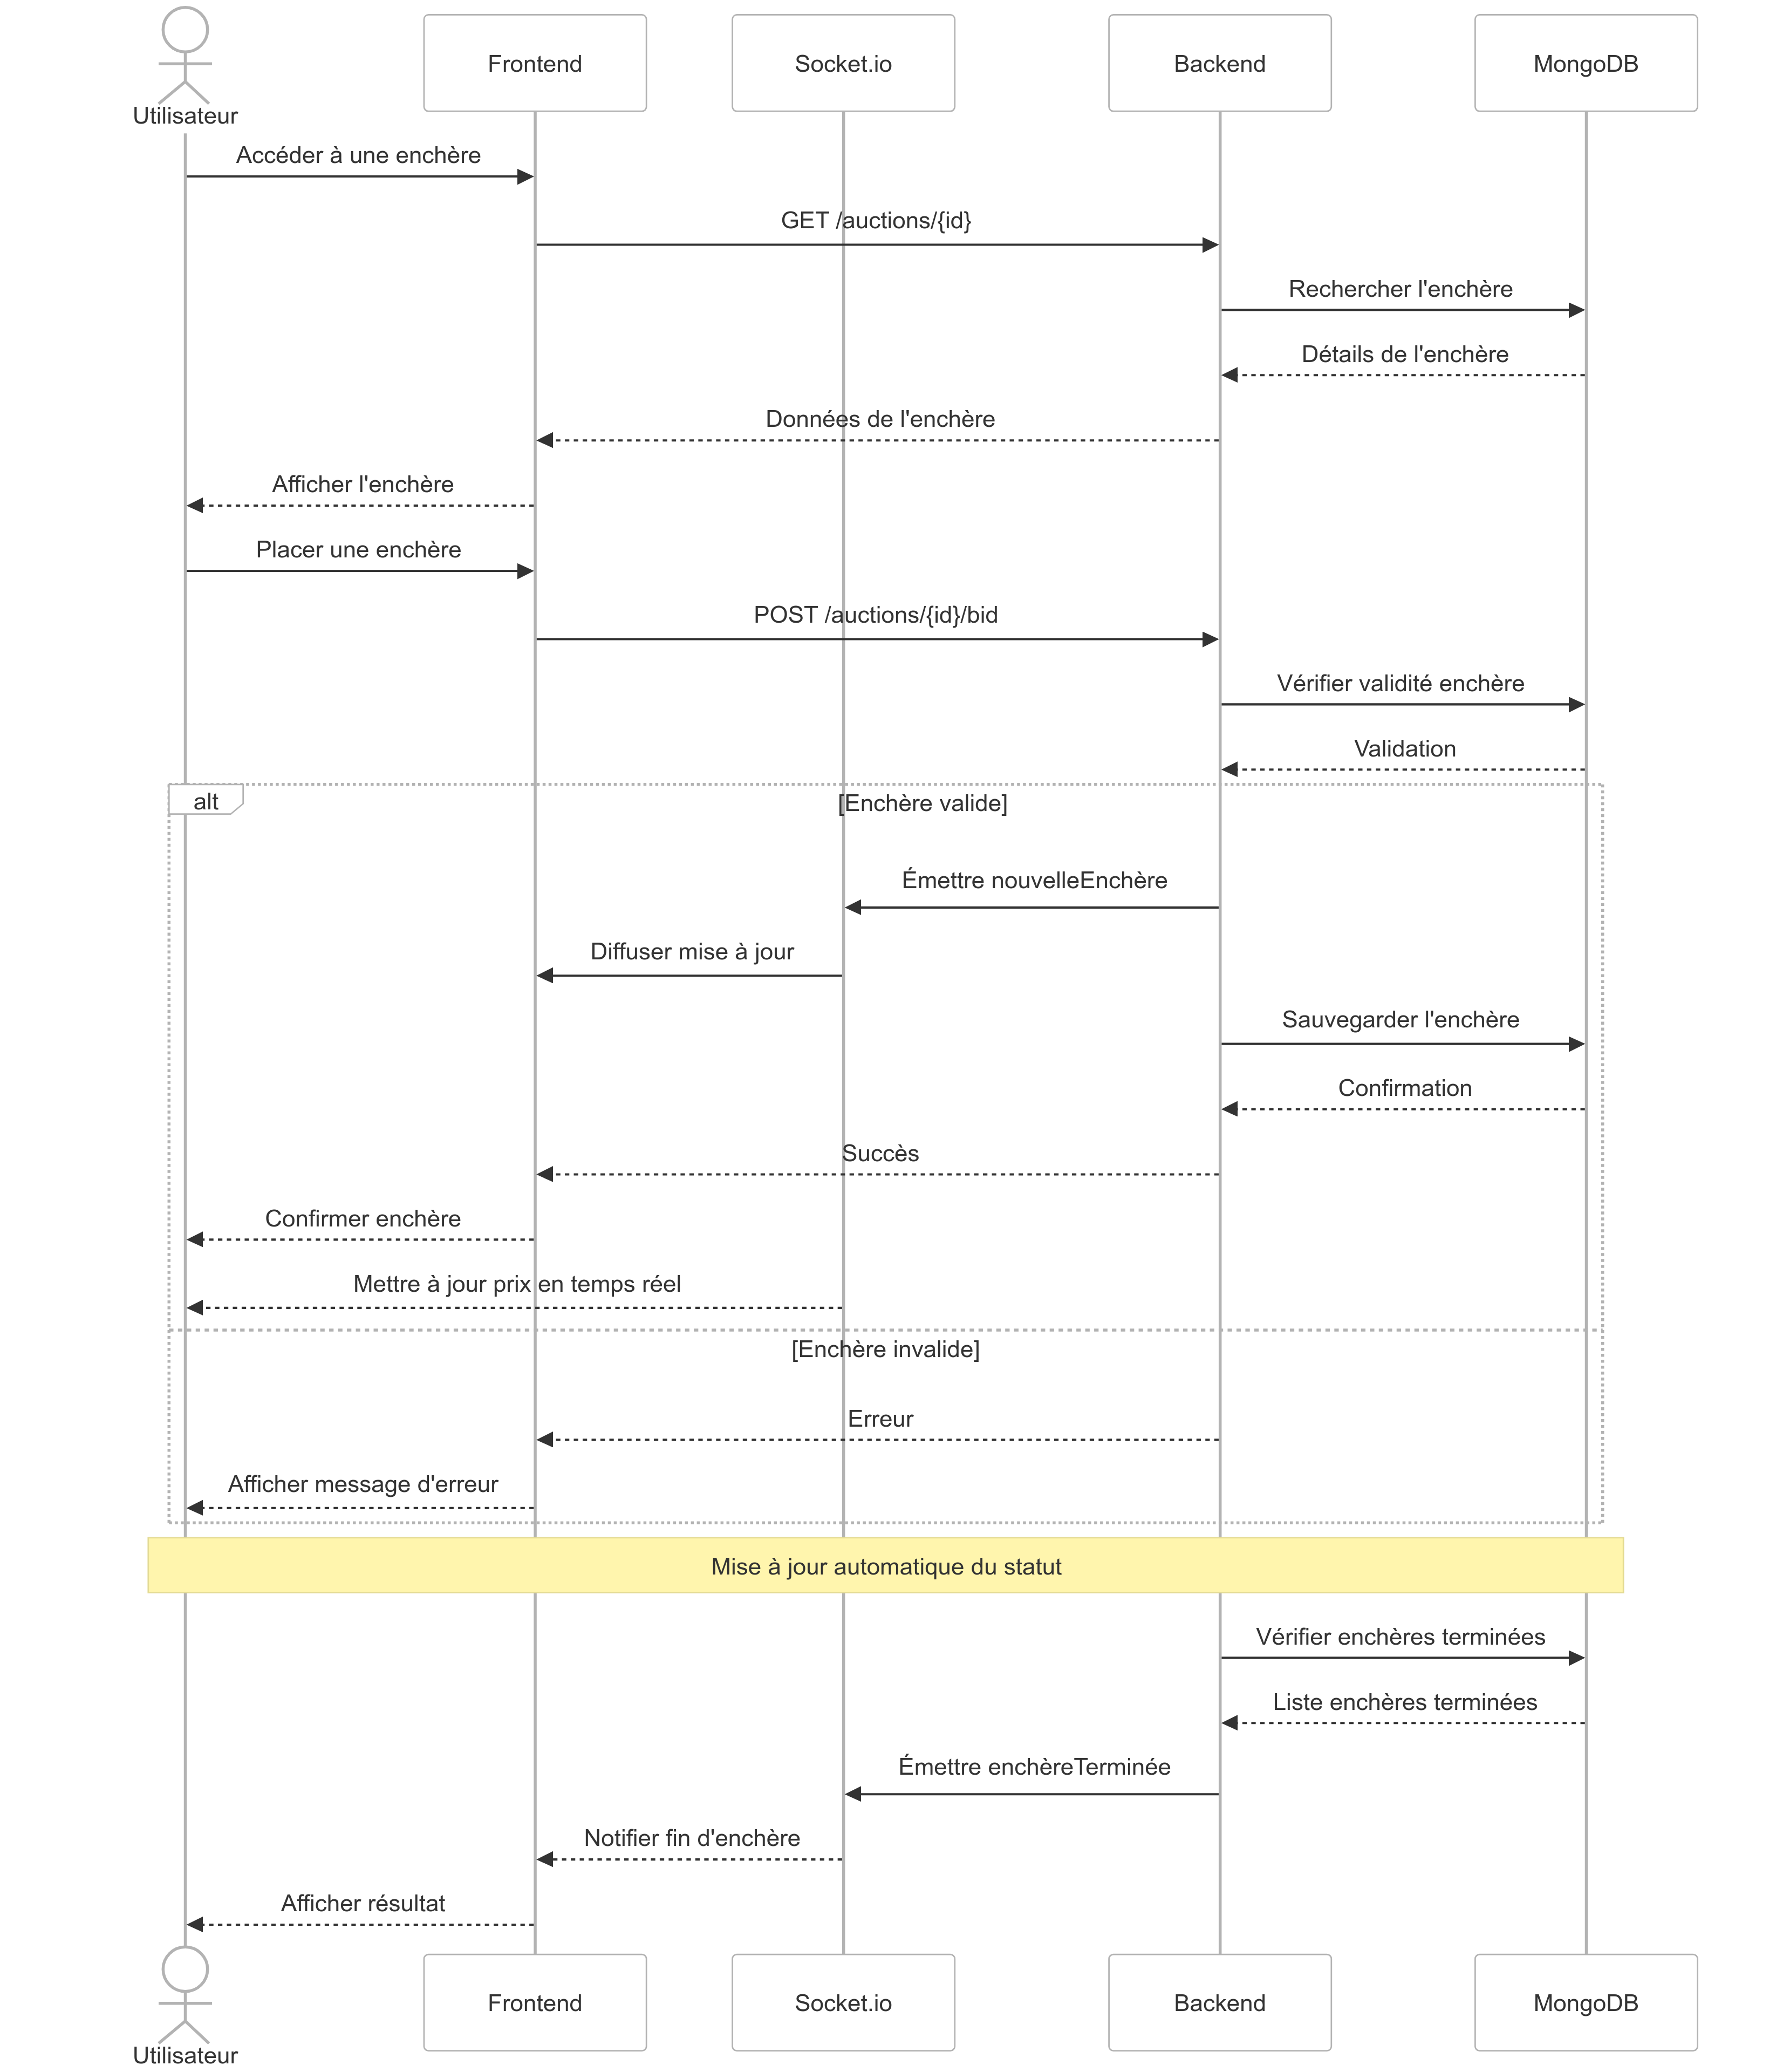
\includegraphics[width=\textwidth]{Editor _ Mermaid Chart-2025-04-03-140837.png}
    \caption{Diagramme de cas d'utilisation du système d'enchères}
    \label{fig:use-case}
\end{figure}

\subsection{Acteurs du Système}
\begin{itemize}
    \item \textbf{Utilisateur}: Représente un client qui peut consulter les enchères, s'inscrire, se connecter, placer des enchères, gérer son profil et suivre ses enchères.
    \item \textbf{Administrateur}: Dispose de privilèges étendus permettant de gérer les voitures, les utilisateurs et créer de nouvelles enchères.
\end{itemize}

\subsection{Cas d'Utilisation Principaux}
\begin{description}
    \item[Consulter les enchères] Permet aux utilisateurs de visualiser toutes les enchères actives.
    \item[S'inscrire] Création d'un nouveau compte utilisateur.
    \item[Se connecter] Authentification dans le système.
    \item[Placer une enchère] Soumettre une offre sur un véhicule en enchère.
    \item[Gérer profil] Modifier les informations personnelles.
    \item[Voir mes enchères] Consulter l'historique personnel des enchères.
    \item[Gérer les voitures] Fonctionnalité réservée à l'administrateur pour ajouter, modifier ou supprimer des véhicules.
    \item[Gérer les utilisateurs] Fonctionnalité réservée à l'administrateur pour gérer les comptes utilisateurs.
    \item[Créer une enchère] Fonctionnalité réservée à l'administrateur pour initier une nouvelle enchère.
\end{description}

\section{Diagramme de Séquence}
Le diagramme de séquence suivant illustre le flux d'interaction entre les différentes composantes du système lors du processus d'enchère.

\begin{figure}[ht]
    \centering
    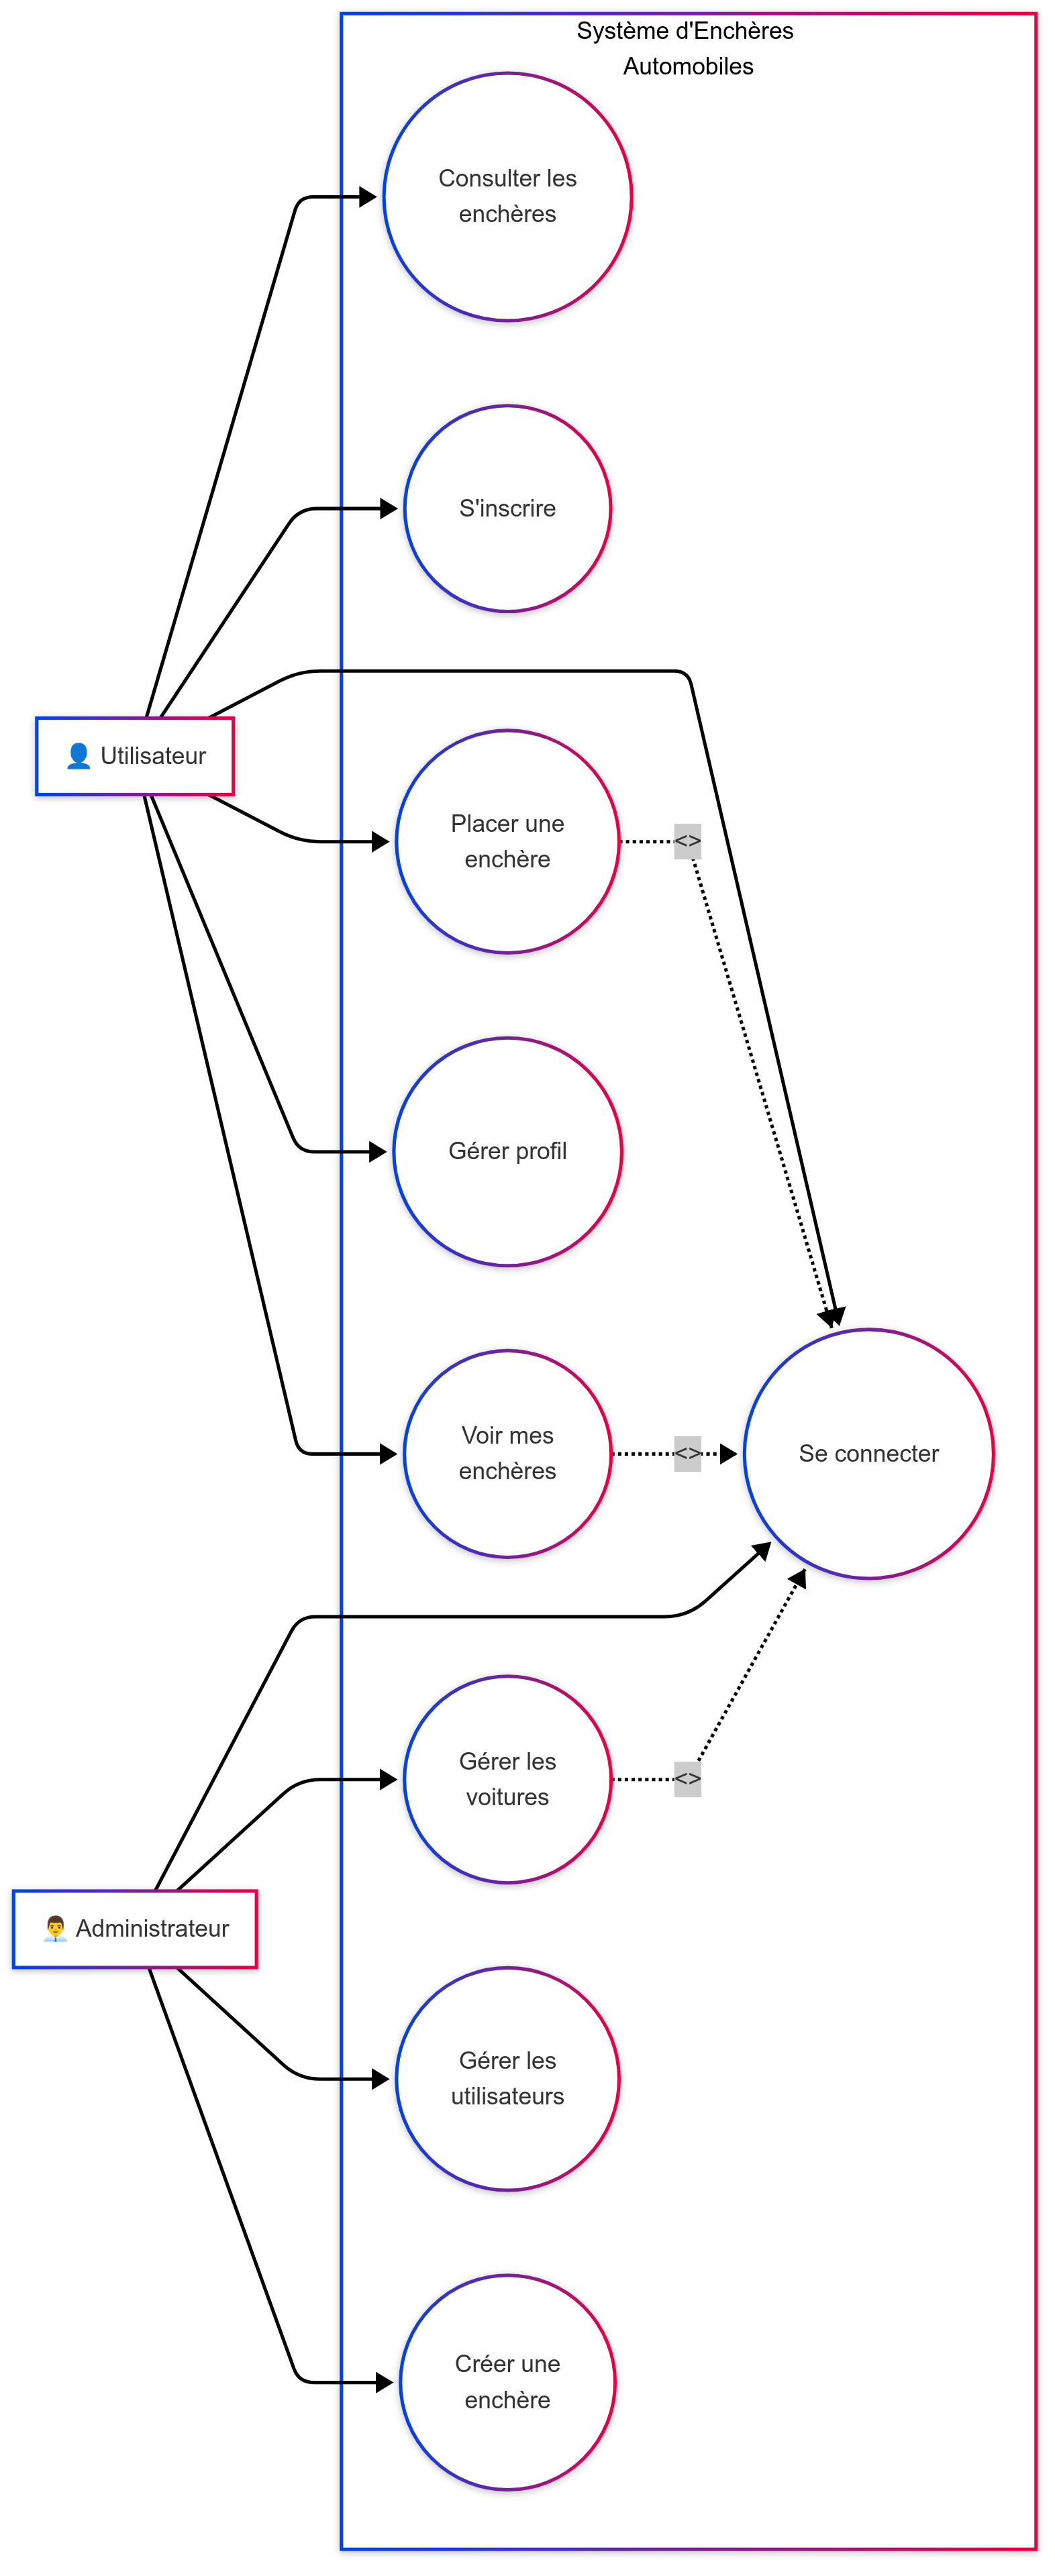
\includegraphics[width=\textwidth]{Editor _ Mermaid Chart-2025-04-03-141556.png}
    \caption{Diagramme de séquence pour le processus d'enchère}
    \label{fig:sequence-diagram}
\end{figure}

\subsection{Analyse du Flux d'Enchère}
Le diagramme de séquence décompose le processus d'enchère en plusieurs étapes clés:

\begin{enumerate}
    \item L'utilisateur accède à une enchère via l'interface frontend
    \item Le frontend demande les détails de l'enchère au backend via une requête GET
    \item Le backend interroge la base de données pour récupérer les informations
    \item L'utilisateur place une enchère qui est envoyée au serveur
    \item Le backend vérifie la validité de l'enchère
    \item Si l'enchère est valide:
    \begin{itemize}
        \item L'enchère est enregistrée dans la base de données
        \item Une notification en temps réel est émise via Socket.io
        \item Tous les clients connectés sont informés de la mise à jour
    \end{itemize}
    \item Si l'enchère est invalide, un message d'erreur est retourné
    \item Le système met à jour automatiquement le statut des enchères terminées
\end{enumerate}

\section{Diagramme de Classes}
Le diagramme de classes suivant représente la structure des entités principales du système et leurs relations.

\begin{figure}[ht]
    \centering
    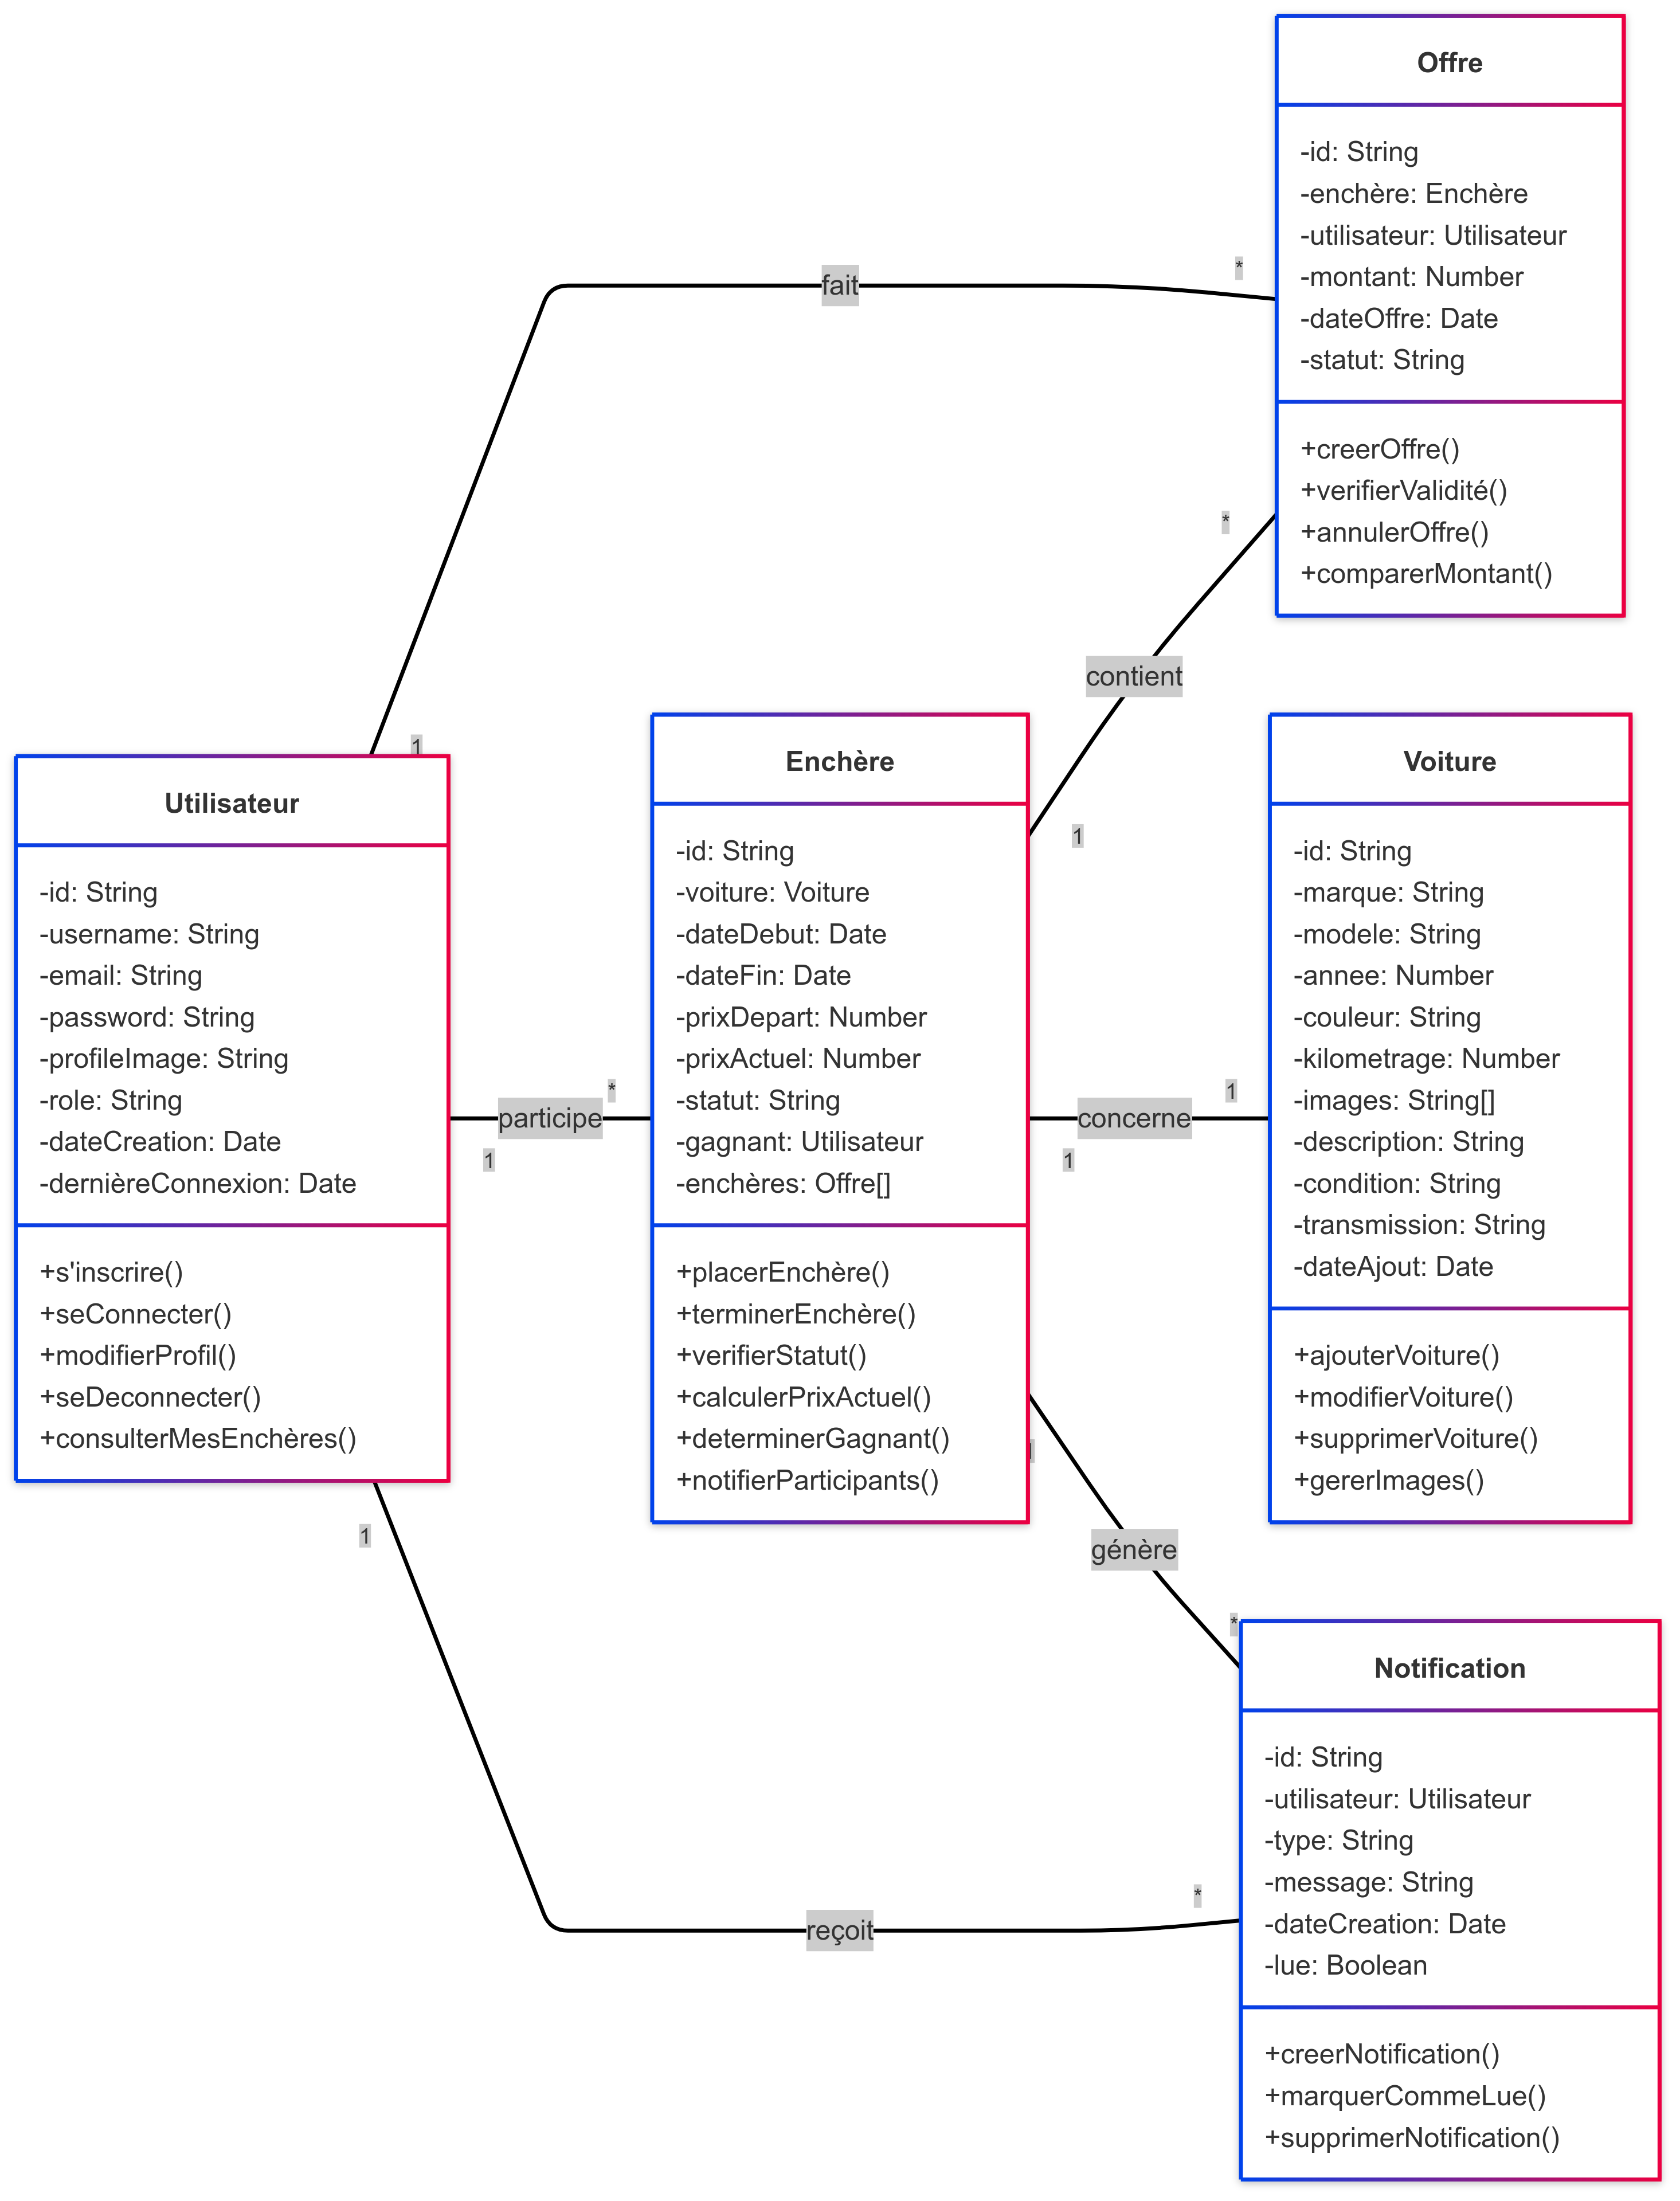
\includegraphics[width=\textwidth]{Editor _ Mermaid Chart-2025-04-03-140758.png}
    \caption{Diagramme de classes des principaux composants du système}
    \label{fig:class-diagram}
\end{figure}

\subsection{Entités Principales}
\begin{description}
    \item[Utilisateur] Contient les informations personnelles et d'authentification. Un utilisateur peut participer à plusieurs enchères et recevoir des notifications.
    \item[Enchère] Représente une session d'enchères avec une date de début, de fin, un prix de départ et un prix actuel. Une enchère concerne un véhicule spécifique et contient plusieurs offres.
    \item[Voiture] Contient les informations détaillées d'un véhicule mis aux enchères, comme la marque, le modèle, l'année, et des images.
    \item[Offre] Représente une proposition financière faite par un utilisateur dans le cadre d'une enchère.
    \item[Notification] Permet d'informer les utilisateurs des événements importants comme les surenchères ou la fin d'une enchère.
\end{description}

\subsection{Relations Entre Entités}
\begin{itemize}
    \item Un utilisateur peut participer à plusieurs enchères (relation n-n)
    \item Une enchère concerne exactement une voiture (relation 1-1)
    \item Un utilisateur peut faire plusieurs offres (relation 1-n)
    \item Une enchère contient plusieurs offres (relation 1-n)
    \item Un utilisateur reçoit plusieurs notifications (relation 1-n)
    \item Une enchère génère plusieurs notifications (relation 1-n)
\end{itemize}

\section{Modèles de Données}

\subsection{Modèle Utilisateur}
\begin{verbatim}
const userSchema = new Schema({
  id: String,
  username: String,
  email: String,
  password: String,
  profileImage: String,
  role: String,
  dateCreation: Date,
  dernièreConnexion: Date
});
\end{verbatim}

\subsection{Modèle Enchère}
\begin{verbatim}
const enchereSchema = new Schema({
  id: String,
  voiture: { type: Schema.Types.ObjectId, ref: 'Voiture' },
  dateDebut: Date,
  dateFin: Date,
  prixDepart: Number,
  prixActuel: Number,
  statut: String,
  gagnant: { type: Schema.Types.ObjectId, ref: 'Utilisateur' },
  encheres: [{ type: Schema.Types.ObjectId, ref: 'Offre' }]
});
\end{verbatim}

\subsection{Modèle Voiture}
\begin{verbatim}
const voitureSchema = new Schema({
  id: String,
  marque: String,
  modele: String,
  annee: Number,
  couleur: String,
  kilometrage: Number,
  images: [String],
  description: String,
  condition: String,
  transmission: String,
  dateAjout: Date
});
\end{verbatim}

\subsection{Modèle Offre}
\begin{verbatim}
const offreSchema = new Schema({
  id: String,
  enchere: { type: Schema.Types.ObjectId, ref: 'Enchere' },
  utilisateur: { type: Schema.Types.ObjectId, ref: 'Utilisateur' },
  montant: Number,
  dateOffre: Date,
  statut: String
});
\end{verbatim}

\section{Architecture Technique}

\subsection{Architecture Frontend}
L'application frontend est développée avec React Native, ce qui permet un déploiement sur iOS et Android à partir d'une base de code unique. Les principales composantes de l'architecture frontend sont:

\begin{itemize}
    \item \textbf{Écrans}: Représentent les différentes vues de l'application
    \item \textbf{Composants}: Éléments d'interface réutilisables
    \item \textbf{Services}: Modules pour la communication avec le backend
    \item \textbf{État global}: Gestion centralisée de l'état de l'application
    \item \textbf{Navigateurs}: Gestion de la navigation entre écrans
\end{itemize}

\subsection{Architecture Backend}
Le backend est construit sur Node.js avec Express.js comme framework web. L'architecture est organisée selon les principes MVC (Modèle-Vue-Contrôleur) adaptés aux API REST:

\begin{itemize}
    \item \textbf{Routes}: Définissent les points d'entrée API
    \item \textbf{Contrôleurs}: Contiennent la logique métier
    \item \textbf{Modèles}: Représentent les entités de base de données
    \item \textbf{Middleware}: Composants pour l'authentification et la validation
    \item \textbf{Services}: Logique partagée entre différents contrôleurs
\end{itemize}

\subsection{Communication en Temps Réel}
La communication en temps réel est gérée par Socket.io, qui permet:

\begin{itemize}
    \item Des mises à jour instantanées des enchères
    \item Des notifications en temps réel pour les utilisateurs
    \item La gestion de salles d'enchères virtuelles
    \item Une reconnexion automatique en cas de perte de connexion
\end{itemize}

\subsection{Base de Données}
MongoDB a été choisi comme système de base de données pour sa flexibilité et sa scalabilité. Les caractéristiques clés de notre implémentation MongoDB sont:

\begin{itemize}
    \item Schémas flexibles permettant une évolution rapide
    \item Relations entre documents gérées par références
    \item Indexation pour optimiser les performances de requête
    \item Agrégations pour des analyses complexes
\end{itemize}